\documentclass[12pt]{exam}

\usepackage{ge13}       % local style file
\usepackage{comment}
\usepackage{graphicx}
\usepackage{hyperref}
\urlstyle{rm}   % change fonts for url's (from Chad Jones)
\hypersetup{
    colorlinks=true,        % kills boxes
    allcolors=blue,
    pdfsubject={NYU Stern course GB 2303, Global Economy},
    pdfauthor={Dave Backus @ NYU},
    pdfstartview={FitH},
    pdfpagemode={UseNone},
%    pdfnewwindow=true,      % links in new window
%    linkcolor=blue,         % color of internal links
%    citecolor=blue,         % color of links to bibliography
%    filecolor=blue,         % color of file links
%    urlcolor=blue           % color of external links
% see:  http://www.tug.org/applications/hyperref/manual.html
}

\usepackage{enumitem}
    \setitemize{leftmargin=*, topsep=0pt}
    \setenumerate{leftmargin=*, topsep=0pt}
\usepackage{attachfile}
    \attachfilesetup{color=0.75 0 0.75}
\usepackage{needspace}
% example:  \needspace{4\baselineskip} makes sure we have four lines available before pagebreak

% for ge13.sty
\def\ClassName{The Global Economy}
\def\Category{Professor David Backus}
\def\HeadName{Problem Set \#1}
\newcommand{\phm}{\phantom{--}}
\newcommand{\NX}{\mbox{\it NX\/}}

% prints answers -- or not, if commented out
\printanswers

\begin{document}
\parindent = 0.0in
\parskip = \bigskipamount
\thispagestyle{empty}%
\Head

\centerline{\large \bf \HeadName: Macroeconomic Data}
\centerline{Revised:  \today}

\medskip
{\it You may do this assignment in a group.
Whatever you hand in should be the work of your group
and include the names of all of the contributors.}

\begin{questions}

\begin{solution}
Brief answers follow,
but see also the attached spreadsheet:
download this pdf file, open it with the Adobe Reader or the equivalent,
and click on the pushpin:
\attachfile{ps1_f13_answerkey.xlsx} \\
{\it Warning:  If you don't see a pushpin above, my guess is you have a Mac.
The pushpin doesn't appear in Preview,
but you can use the Adobe Reader or the equivalent.}
\end{solution}


% --------------------------------------------------------------------
\question {\it National accounts in Margaritaville (40 points).\/}
Jimmy Buffett has decided to apply for membership in the European Union
on behalf of his newly sovereign nation, Margaritaville.
As part of his application, he must provide the EU
technocrats with a complete set of national accounts.
You have been hired as the Chief National Accountant.
Your first day on the job,
you receive an official Coral Reefer Crew{\texttrademark} t-shirt
and the following information about local economic activity:
%
\begin{itemize}
\item Local Cheeseburger in Paradise{\texttrademark} cafes
sold \$63,000 worth of cheeseburgers to local consumers.
Their expenses were:  imported beef and sesame seeds (\$10,000),
locally produced catsup (\$12,000),
wages and benefits (\$22,000), and rent (\$3,000).
Hint: you will need to compute the profit earned by the cafes.

\item Local tomato growers sold \$8,000 worth of tomatoes to domestic
catsup producers and exported another \$3,000 to the US.
They paid land rent (\$1,000) and wages (\$9,000).

\item Local producers of the Margaritaville Frozen Concoction Maker{\texttrademark }
sold \\ \$100,000 worth of blenders;
40\% were exported to Europe, the remainder to local consumers.
Their expenses were \$15,000 worth of imported metal,
\$20,000 for a new CNC machine imported from Germany,
and \$70,000 in wages.

\item The domestic catsup industry sold \$12,000 worth of product to local
cafes.
They purchased \$8,000 worth of tomatoes from domestic growers
and paid \$4,000 in wages.


\item The newly-formed government collected \$10,000 in taxes from its citizens
and paid \$10,000 to government regulators, who oversee food and beverage safety.
\end{itemize}
%
You mission is to use this raw data to construct
national income and product accounts for Magaritaville.
Specifically:
%
\begin{parts}
\part Compute the value-added of each production unit.
What is GDP?
(10~points)

\part Compute GDP and its expenditure components (consumption,
investment, government purchases of goods and services,
exports, and imports).
(10~points)

\part What are saving and investment?  Why are they different?
Where does the difference go?
(10~points)

\part Jimmy looks over your calculation in (a) and is worried
that you made a mistake.
Over a couple Land Shark Lagers{\texttrademark}
you explain to him that GDP can be computed three different ways:
the sum of value-added across production units (Gross Domestic Product),
the sum of expenditure components (Gross Domestic Expenditure),
and the sum of payments to labor and capital (Gross Domestic Income).
You do the remaining one, payments to labor and capital,
and show him that you get the same answer.
He buys you a margarita to show his appreciation.
(10~points)
\end{parts}

\begin{solution}
It's easiest to do the whole thing on a spreadsheet --- see the link on
the course website.
The idea is to calculate value added, income, and final sales,
as we did in class.
It includes government production,
which is valued at cost (income = value added),
investment,
which is not counted as an expense,
and imports.

\begin{parts}
\part Here's a quick overview of value added by producer:
\begin{itemize}
\item Cafes:  Value added comes from
sales of 63 minus intermediate goods of 22,
which gives you value-added of 41.
On the income side this corresponds to 22 to labor, 3 in rent, and 16 of profit
to the owner.
\item Tomatoes:  Value added is 11, which equals
income of 11 (9 to labor, 1 to rent, 1 of profit).
\item MFCM:  Value added is sales of 100 minus the 15 of metal,
for a total of 85.
By convention, we do not include the 20 of new machines as an expense,
because it's an investment in new plant and equipment.
On the income side, that consists of wages of 70 and profit of 15.
\item Catsup:  Revenue of 12 minus intermediate inputs of 8
gives us value-added of 4, which is paid as wages.
\item Government.  Wages of 10 count (by convention) as value added of 10,
all of it income to government workers.
\end{itemize}
Adding it all up gives us GDP from the production side:
\begin{eqnarray*}
        \mbox{Value added}  &=& 41 + 11 + 85 + 4 + 10 \;\;=\;\; 151 .
\end{eqnarray*}

\part Expenditures are
\begin{itemize}
\item Cafes:  All of the sales revenue is final sales to consumers.
How do we handle the input of imported beef and seeds?
We put a 10 in imports, which therefore makes a negative
contribution to expenditures on (our) GDP.
\item Tomatoes:  Only the exports of 3 counts as final sales,
the rest is an input to the catsup producer.
\item MFCM:
Finals sales includes consumption of 60, exports of 40, imports of 35,
and investment of 20.
Note that the investment of 20 makes no contribution to GDP:  the entries
under investment and imports net to zero.
\item Catsup:  None of it counts as final sales, since it's sold to cafes
and used by them as an intermediate product (an input).
\item Government.  Government purchases are 10:
by convention, it ``purchases'' what it produces.
\end{itemize}
Adding it all up gives us GDP from the expenditure identity:
\begin{eqnarray*}
    Y (\mbox{GDP} = 151) &=& C (123) + I (20) + G (10) + \NX (43-45) .
\end{eqnarray*}
\part From above, saving is $S = Y - C - G = 18$ and investment is $I = 20$.
Net exports of $\NX = -2$ accounts for the difference:  $ S = I + \NX$.
In this case, it means we are borrowing 2 in foreign capital markets:
domestic saving is less than we need to finance domestic investment,
so we make up the difference by raising money from foreign investors.
\part We've calculated GDP from value-added of producers and expenditures.
The only one we're missing is income, which (of course)
is the same as value added.
Summing again across production
units in order of appearance:
\begin{eqnarray*}
       \mbox{Gross Domestic Income} &=&  41 + 11 + 85 + 4 + 10 \;\;=\;\; 151 .
\end{eqnarray*}
This breaks down into wages (115), rent (4), and profit (32).
Thus we have three ways to get the same number:  value added, expenditures, and income.
The numbers are all the same, so we can drink our margarita in peace.

\end{parts}
\end{solution}

%\begin{comment}
% --------------------------------------------------------------------
\question {\it Inputs and outputs (20 points).\/}
Specify the most likely direct impact of each of the following
on the components of the production function.
Don't make this more complicated than it is:
we're concerned only with
the impact on the components of the production function.
%
\begin{parts}
\part A ``ghost city'' in China, complete with new office and apartment buildings,
but with no people. (5~points)
\part A reduction in the employer tax on workers that leads firms to hire more people. (5~points)
\part An improvement in education that increases the skill and effectiveness of workers. (5~points)
\part A reduction in tariffs in Brazil on imported computer equipment. (5~points)
\end{parts}

\begin{solution}
You may recall that the production function links output $Y$
to inputs of capital $K$ and labor $L$ and productivity $A$:
\begin{eqnarray*}
    Y &=& A K^{1/3} L^{2/3} .
\end{eqnarray*}
\begin{parts}
\part This is an increase in capital,
but since it's not used, it generates no additional output.
To make this work in the production function, we need productivity to fall.

Update:  some people have suggested that stories about these ghost cities are overblown, 
perhaps completely wrong.  
See
\url{http://blogs.wsj.com/chinarealtime/2013/09/24/chinas-ghost-cities-may-not-be-so-spooky/}

\part An increase in labor, which should raise output.
\part This raises the quality-adjusted amount of labor, therefore output goes up.
If labor is measured without quality adjustment, then it shows up as an increase in productivity.
As usual, productivity absorbs anything that's not accounted for explicitly.
\part This makes computer equipment cheaper, which should increase the capital
stock and thus output.
It could also raise productivity
by giving Brazilian firms cheaper/better access to the best computer technology.

From a paper by Cole, Ohanian, Riascos, and Schmitz (``Latin America
in the rearview mirror'') (rough paraphrase):
\begin{quote}
In 1977, Brazil embarked on a zero-quota policy that
meant that only PCs and minicomputers produced by Brazilian-owned firms
could be sold in Brazil.
Moreover, the black market was not a practical choice for large firms.
The policy insulated Brazilian computer producers from foreign competition
and featured entry barriers to new Brazilian producers through
a maze of bureaucratic requirements.

When the quota was lifted by President Collor in 1992,
productivity in Brazil's computer industry rose dramatically
and 6 of the top 10 firms selling in Brazil in the mid-1990s were
Brazilian.
Productivity of computer users also increased,
as firms got access to better equipment at lower prices.
\end{quote}
\end{parts}
\end{solution}

% --------------------------------------------------------------------
\question {\it Saving, investment, and capital flows in Germany (40~points).\/}
Germany is known for its high saving rate, which has been consistently above
the US rate.
Does this saving support a similarly high investment rate --- or something else?

We'll attack this question with the data in the spreadsheet
attached below to the pdf of this document,
linked on the course page, and posted at

\vspace*{\parskip}
\centerline{\url{http://pages.stern.nyu.edu/~dbackus/2303/ps1_q3_f13.xls}.}

The first sheet, labeled {\tt Data}, includes everything you need:
GDP and its expenditure components at current prices from 1980 to 2013 (estimated).
The second contains the data exactly as it comes
from the EIU's CountryData and can be ignored.
Note the discrepancies in the 1980s:
they're small, fortunately, but they tell us the expenditure identity
doesn't quite work here, the numbers are internally inconsistent.
Disappointing, but that's the real world for you.

\begin{parts}
\part What does ``GDP at current prices'' mean?
Is it ``real'' or ``nominal''?
What do those words mean anyway?
(10~points)

%\part Check the expenditure identity, $ Y = C + I + G + \NX$.
%Why isn't it satisfied here?
%(10~points)

\part Graph saving, investment, and net exports as ratios to GDP.
How are these three variables related?
As in class, we define saving as $S = Y - C - G $.
By convention, investment includes both ``gross fixed investment''
and ``stockbuilding'' (accumulation of inventories).
(20~points)

\item Looking at your figure,
how much of domestic saving is used to finance domestic investment?
What happens to the rest of it?
(10~points)
\end{parts}

{\it Data file (download pdf, open, click on pushpin): }
\attachfile{ps1_q3_f13.xls}

\begin{solution}
\begin{parts}
\item When we measure something ``at current prices''
we say it's a {\it nominal\/} magnitude, measured in units of money.
When we measure something ``at constant prices,''
we say it's a {\it real\/} magnitude.
Since the prices are the same at all dates,
all of the variation over time in real magnitudes is in the quantities.
So real GDP measures the quantity of goods and services produced
and nominal GDP measures their value (prices times quantity)
in units of currency.

\item Here's the graph:
\begin{center}
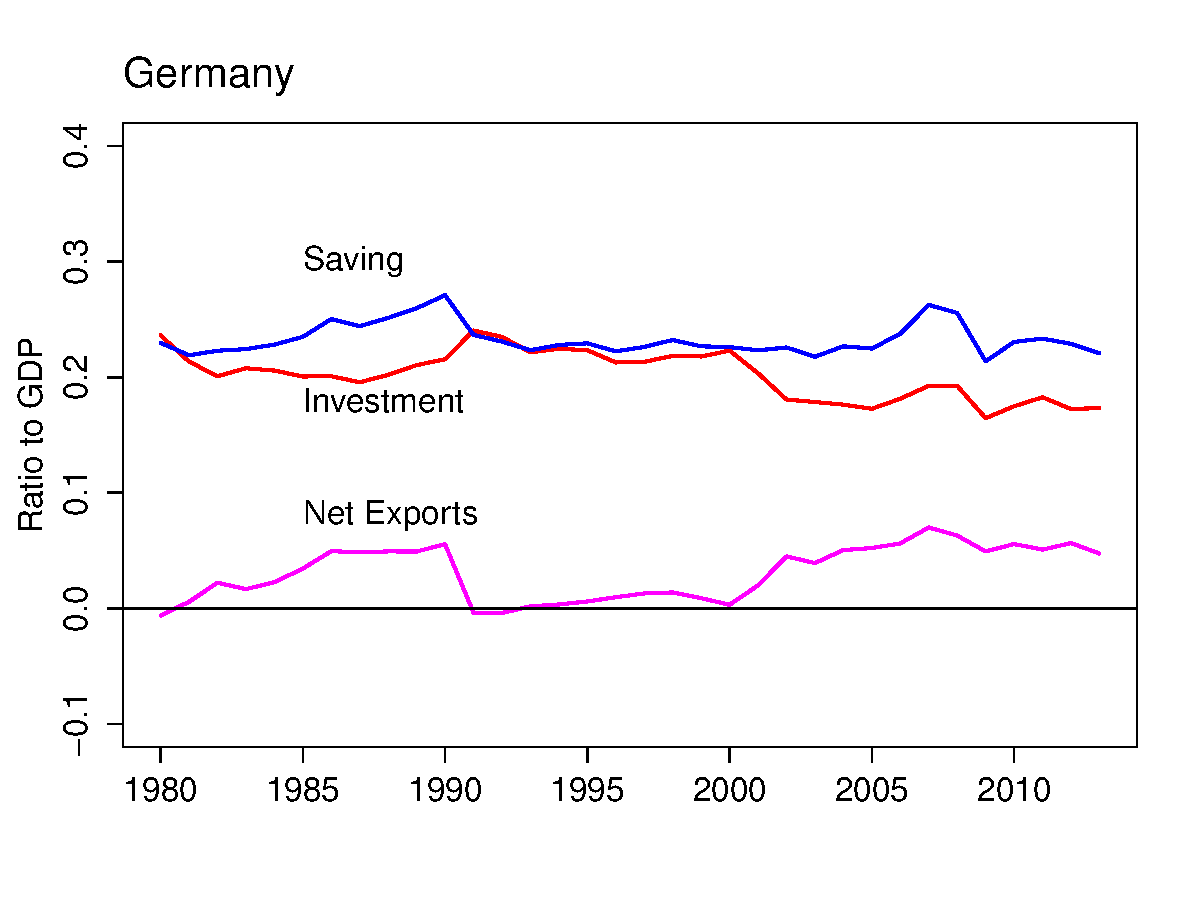
\includegraphics[scale=0.5]{Germany_shares.pdf}
\end{center}
%
The variables are related by
\begin{eqnarray*}
        S &=& Y - C - G \;\;=\;\; I + \NX .
\end{eqnarray*}
(Well, they would be if not for the discrepancy.)

{\it For experts only, here's the R file that produced the figure
(R is a popular open source statistics program)
(download pdf, open, click on pushpin): }
\attachfile{ps1_f13.R}


\item The point here is that net exports reflects international
movements of capital.
If $\NX > 0$,  we have more saving
than investment and the extra funds are invested abroad as
a ``capital outflow.''
If $\NX < 0$,  we have more investment than saving
and the difference is made up by raising money abroad ---
what we call a ``capital inflow.''
In the recent past, Germany has experienced a capital outflow,
largely because investment has fallen.
The excess saving is then channelled into foreign investments.

This goes beyond the question, but you'll see two interpretations
of such capital inflows.
One is that the country must be doing well to attract capital from abroad.
The other is that the country must be doing poorly because it's had to borrow.
There is, unfortunately, no simple answer to which it is.
%More later in the course.

\end{parts}
\end{solution}
\end{questions}

%{\it Data file for Question 3 (download pdf, open, click on pushpin): }
%\attachfile{ps1_q3_f13.xls}


\vfill \centerline{\it \copyright \ \number\year \
NYU Stern School of Business}

\end{document}

